%%%%%%%%%%%%%%%%%%%%%%%%%%%%%%%%%%%%%%%%%%%%%%%%%%%%%%%%%%%%%%%%%%%%%%%%%%%

\documentclass[a4paper,oneside,12pt]{article}
\usepackage{mystyle}

\begin{document}

\title{\Large\bf Quadratic functions}
\author{%%
  Minh Van Nguyen \\
  \url{mvngu@gmx.com}
}
\date{\today}
\maketitle

\begin{packeditem}
\item General quadratic function.

\item Graph of quadratic function.

\item Factoring quadratic function.

\item Completing the square.

\item Application: gravity and displacement of projectile.

\item Area under a quadratic function.
\end{packeditem}


%%%%%%%%%%%%%%%%%%%%%%%%%%%%%%%%%%%%%%%%%%%%%%%%%%%%%%%%%%%%%%%%%%%%%%%%%%%

\section{General form}

A \emph{quadratic function} is an equation of the form
%%
\begin{equation}
\label{eqn:general_quadratic_function}
f(x)
=
ax^2 + bx + c
\end{equation}
%%
where $\triple{a}{b}{c} \in \RR$ are known constants and $x$ is a
variable that can be any real number.  What does the function $f(x)$
look like?

As an example, set $a = 1$ and $b = c = 0$ in
\Equation{eqn:general_quadratic_function} so that you have
$f(x) = x^2$.  Let's calculate the function value for
$x = \sextuple{-4}{-3}{-2}{2}{3}{4}$.  Note that you have
\[
f(2) = f(-2) = 4,
%%
\quad
%%
f(3) = f(-3) = 9,
%%
\quad
%%
f(4) = f(-4) = 16.
\]
Plot these points on one set of coordinate axes and draw a line
through the points to get the graph in \Figure{fig:quadratic_a_1}.
Note that $f(0) = 0$ so the graph of $f(x) = x^2$ touches the origin.
The general shape of the graph of
\Equation{eqn:general_quadratic_function} looks like the beak of a
duck~(or some other bird) and the usual name for this is a
\emph{parabola}.

\begin{figure}[!htbp]
\centering
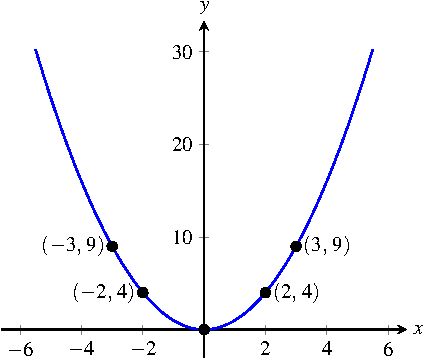
\includegraphics[scale=1.2]{image/07/a-1.pdf}
\caption{%%
  A graph of the function $f(x) = x^2$.  The general shape of the
  graph is called a \emph{parabola}.
}
\label{fig:quadratic_a_1}
\end{figure}

Generally speaking, how would you draw the graph of
\Equation{eqn:general_quadratic_function}?  One way is to start at the
tip of the parabola and choose a few values of $x$ that are equally
spaced.  If the tip of the parabola is $\tuple{a}{b}$, the following
values of $x$
\[
\septuple{a-3}{a-2}{a-1}{a}{a+1}{a+2}{a+3}
\]
should usually be good enough for a rough sketch of the graph of
\Equation{eqn:general_quadratic_function}.  Of course, you still need
to calculate the function values $f(a-3)$, $f(a-2)$, $f(a-1)$,
$f(a+1)$, $f(a+2)$, and $f(a+3)$.  Note that the graph of the
quadratic function $f(x)$ is symmetric about the tip point
$\tuple{a}{b}$.  This means that
\[
f(a+1) = f(a-1),
%%
\quad
%%
f(a+2) = f(a-2),
%%
\quad
%%
f(a+3) = f(a-3)
\]
and so you only need to calculate three function values, not six.
The above strategy is illustrated
in \Figure{fig:sketch_parabola}.

\begin{figure}[!htbp]
\centering
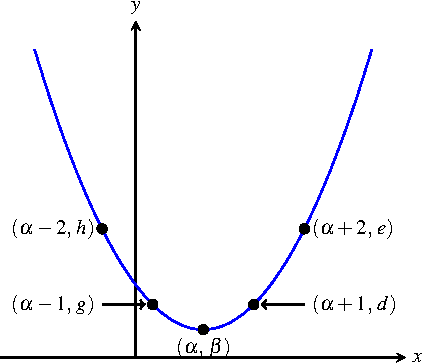
\includegraphics[scale=1.2]{image/07/a1-bminus4-c10.pdf}
\caption{%%
  Sketching the graph of a quadratic function.  First, locate the tip
  $\tuple{a}{b}$ of the function.  From there, spread outward with a
  few points.  Finally, you connect the dots.
}
\label{fig:sketch_parabola}
\end{figure}

The problem now is: How do you calculate the tip of the parabola?  If
you have a quadratic function of the form $f(x) = ax^2 + bx + c$, the
tip of the function is located at the $x$-coordinate
%%
\begin{equation}
\label{eqn:parabola_tip_x_coordinate}
x
=
-\frac{b}{2a}.
\end{equation}
%%
Substitute \Expression{eqn:parabola_tip_x_coordinate} into the
function $f(x)$ to obtain the corresponding $y$-coordinate.  For now,
do not worry about how \Expression{eqn:parabola_tip_x_coordinate} was
derived.  This will be shown later on.

\end{document}
